\chapter{PLSound}


\paragraph{Motivation}
PixelLight itself has NO own sound implementation nor even fixed build in sound support within the scene graph itself. But there are ton's of sound libraries out there - many of them free or even open source. As mentioned before, PixelLight does not come with native sound support - but through the carefully considered design of the PixelLight framework such an 'hacked in'-support is unnecessary, it would even waste the sweet universal design. Because of the extreme plugin nature of PixelLight, it's no problem to add something like sounds to your projects.

The PixelLight SDK itself comes with a few such sound plugins. By using this plugins it's extremely simple to add sound to your scene. In fact, this plugins only have one scene node container for the sound world and a few scene node modifier. Create a scene container using such a sound world scene node container class and add some scene nodes into it. For nodes which should have sound behaviour just add a sound modifier to the node.

You can use multiple sound API's within your project at the same time, but this isn't recommended and doesn't make much sense. So, for your project, you normally have to choose ONE sound API and use it for the hole project. You can extent this PixelLight sound plugins by self (not recommended) or add a plugin for another sound API if required.


\paragraph{External Dependences}
\emph{PLSound} depends on the \textbf{PLScene} library, and therefore an all other libraries \textbf{PLScene} depends on.




% Include the other sections of the chapter
\chapter{Sound}




\section{Overview}
In PixelLight there's no difference between sound and music. Therefore we use only the term sound. The sound component is using backends like the renderer component to enable you to use whatever sound API you want to use. But unlike the renderer component no other PixelLight component depends on the sound component. It's possible to playback 2D and 3D sounds and different sounds and music can be mixed/blended together. Here's a digram the sound component look's like:\\
\begin{figure}
  \begin{center}
    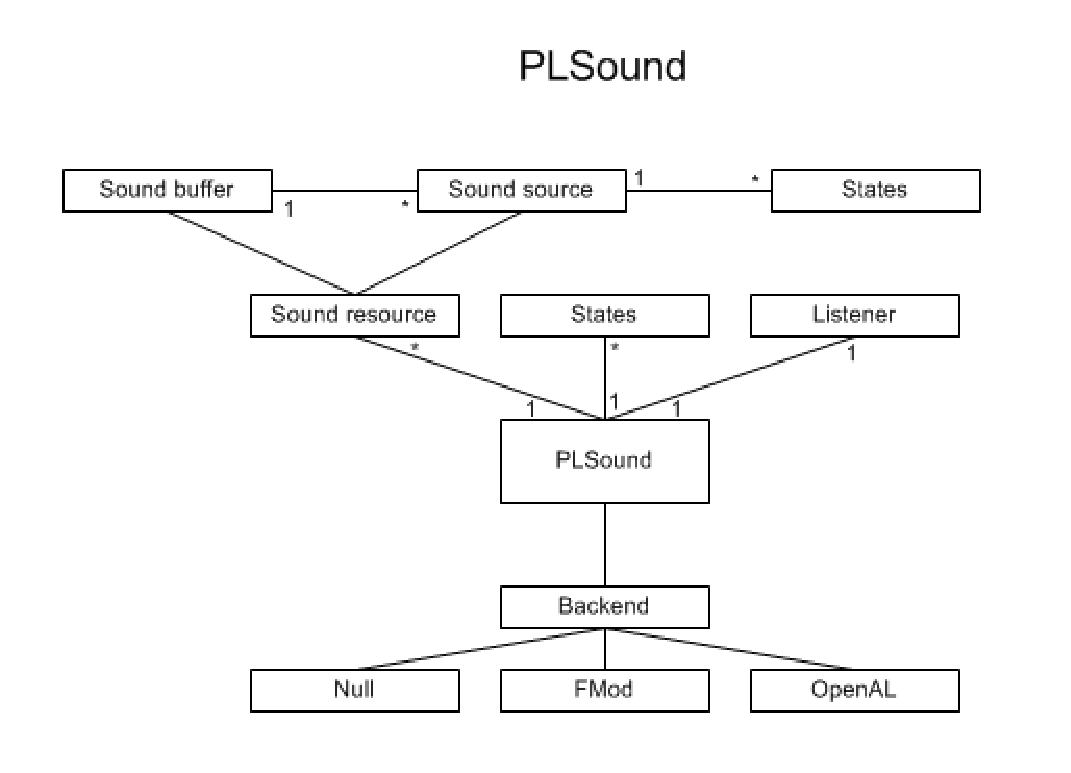
\includegraphics{pics/PLSoundClassDiagram.eps}
  \end{center}
  \caption{Sound component}
  \label{fig:Sound component high-level UML class diagram}
\end{figure}




\section{Sound scene node}
The sound component comes with a scene node called \emph{PLSound::SNSound} you can place into your scene for sound playback. There's also a scene node modifier called \emph{PLSound::SNMSound} if you just want to add sound to a scene node without adding a new one. The sound position is set by this scene node and will do all the dirty work for you, quite easy to deal with dynamic 3D sounds, eh?

This scene plugins can only be used correctly if they are placed inside a \emph{PLSound::SCSound} scene container - but it's not required that they are direct children and can be placed within any sub-container that's inside a sound scene container.

Have a look at the \emph{PLDemoSoundBasic} demo that comes with the PixelLight SDK.

\section{Sound Backends}
This section deals with the different sound backends shipping with the PixelLight SDK.


\paragraph{Null}
\begin{itemize}
\item The null sound backend does nothing - can be useful if you e.g. are in debug mode and don't want to hear any sounds.
\item PixelLight component name: PLSoundNull
\item Used dll's: \emph{PLSoundNull.dll}
\end{itemize}


\paragraph{OpenAL}
\begin{itemize}
\item OpenAL\footnote{OpenAL can be downloaded from \url{http://www.openal.org/}} backend with support of wav and ogg vorbis (streaming/no streaming) is provided.
\item PixelLight component name: PLSoundOpenAL
\item Used dll's: \emph{PLSoundOpenAL.dll}, \emph{OpenAL32.dll} and \emph{wrap\_oal.dll}
\end{itemize}


\paragraph{FMODEx}
\begin{itemize}
\item Currently not within the official PixelLight SDK
\item FMODEx\footnote{FMODEx can be downloaded from \url{http://www.fmod.org/}, only free for none commercial projects, \emph{FMOD Sound System, copyright � Firelight Technologies Pty, Ltd., 1994-2011.}} backend which can produce a lot of state of the art sound effects! Some of many supported formats are mp3, wav, mid, midi, it, mod, s3m, xm etc. 
\item PixelLight component name: PLSoundFMODEx
\item Used dll's: \emph{PLSoundFMODEx.dll} and \emph{fmodex.dll}
\end{itemize}


\paragraph{FMOD}
\begin{itemize}
\item Currently not within the official PixelLight SDK
\item FMOD\footnote{FMOD can be downloaded from \url{http://www.fmod.org/}, only free for none commercial projects, \emph{FMOD Sound System, copyright � Firelight Technologies Pty, Ltd., 1994-2011.}} backend which can produce a lot of state of the art sound effects! Some of many supported formats are mp3, wav, mid, midi, it, mod, s3m, xm etc. 
FMOD is the predecessor of FMODEx. Use the newer FMODEx if possible.
\item PixelLight component name: PLSoundFMOD
\item Used dll's: \emph{PLSoundFMOD.dll} and \emph{fmod.dll}
\end{itemize}

\cleardoublepage
